\documentclass[11pt]{article}

\usepackage{geometry}                % See geometry.pdf to learn the layout options. There are lots.
\geometry{letterpaper}                   % ... or a4paper or a5paper or ... 
%\geometry{landscape}                % Activate for for rotated page \

%\usepackage[parfill]{parskip}    % Activate to begin paragraphs with an empty line rather than an indent

% load two different graphics packages:
\usepackage{graphicx,epsfig}
\usepackage[procnames]{listings} 
\usepackage{float}

\usepackage{amssymb}
\usepackage{amsmath}
\usepackage{mathtools}
\usepackage[square]{natbib}

\usepackage[english]{babel}

\usepackage{showlabels}
\showlabelsinline

\usepackage{xcolor}
\numberwithin{equation}{section}



%\usepackage{epstopdf}
%\DeclareGraphicsRule{.tif}{png}{.png}{`convert #1 `dirname #1`/`basename #1 .tif`.png}

\title{Derivation of the angular momentum budget in spherical pressure coordinates for Reanalysis datasets}
\author{Momme Hell, SIO}
\date{March 14th, 2019}      % Activate to display a given date or no date

%% Some user defined shortcuts to save typing
\newcommand{\ep}{\epsilon}
\newcommand{\beq}{\begin{equation}}
\newcommand{\eeq}{\end{equation}}

\newcommand{\beqs}{\begin{equation*}}
\newcommand{\eeqs}{\end{equation*}}

\newcommand{\dd}{\mathrm{d}}
\newcommand{\ii}{\mathrm{i}}
\newcommand{\ee}{\mathrm{e}}
\newcommand{\goto}{\rightarrow}

\newcommand{\la}{\langle}
\newcommand{\ra}{\rangle}
\newcommand{\defn}{\stackrel{\text{def}}{=}}
\newcommand{\HH}{\mathcal{H}}
\newcommand{\vect}[1]{\boldsymbol{#1}}
\newcommand{\Dt}[1]{\frac{D#1}{D t}}

\newcommand{\lara}[1]{\left\la{#1}\right\ra}
\newcommand{\cphi}{\cos \phi}
\newcommand{\rb}{\rho_\beta}

\newcommand{\barsharp}[1]{\overline{#1}^\sharp}



\newcommand{\comment}[1]{{\color{red}[#1]}}

\begin{document}
\maketitle

\section{Introduction}
The atmospheric momentum budget is derived in spherical pressure coordinates and formalted  such that it can be calculated from reanalysis data.\par

The relation of the angular momentum (AM) budget, the zonal momentum equation and eddy-fluxes are in \citet[chapter 11,][]{Peixoto2008}. A shorter introduction in the governing equations is given \citet[chapter 4.12, and 13.10,][]{Gill1982} as well as \citet{Andrews1987} or even \citet{Holton1975}.\par

Section 2 of this manual introduces the AM-equation, section 3 and 4 explain simplifications due to averaging and section 5 introduces the difficulties of the budget in pressure coordinates. Section 6 explains how to apply this algebraic exercise to ERA5 data. 

\section{The governing Angular Momentum equation}
The Angular Momentum (AM) is defined as 

\beq
M = M_\Omega + M_r ~=~ \Omega r^2 \cos^2 \phi + u r\cos \phi, 
\eeq

where $\Omega$ is the earth rotation rate, $u$ the zonal wind, and $r$ the mean earth radius. Errors due to the variation of $r$ is generally small, though largest in the stratosphere (about $1\%$ following \citet[][chapter 4.12, p.93]{Gill1982}. $M_\Omega$ is the Angular Momentum of the atmosphere as it would be in solid rotation with earth, while $M_r$ is the movement relative to the earth rotation.\par

The balance equation for angular momentum per unit volume in the rotating frame with longitude $\lambda$, latitude $\phi$ and height $z$ is  
\beq
\rho \Dt M = - \frac{\partial~p}{\partial \lambda} + \rho~F_\lambda~ r \cphi, 
\eeq
where $p$ is the pressure, $\rho$ is the density, $F_\lambda$ the frictional torques \citep[eq. 11.4,][]{Peixoto2008}. The Total derivate is 
\beq
\Dt~(\cdot) = \frac{\partial}{\partial t} (\cdot) + u~ \frac{\partial}{r \cphi ~\partial \lambda}  (\cdot) + v~ \frac{\partial}{r~ \partial \phi} (\cdot) + w ~ \frac{\partial}{\partial z}  (\cdot).
\eeq


The divergence operator of a vector field $\vect a$ is 

\beq
div(\vect a ) = \frac{\partial}{\partial z} a_z + \frac{2 a_z}{r} + \frac{1}{r \cos{\phi}}  \frac{\partial}{\partial \phi} ( a_{\phi} \cos{\phi}) + \frac{1}{r \cos{\phi}} \frac{\partial}{\partial \lambda} a_\lambda, 
\eeq
(or in pressure coordinates
\beq
div(\vect a ) = - g \frac{\partial}{\partial p } \rho a_z + \frac{2 a_z}{r} + \frac{1}{r \cos{\phi}}  \frac{\partial}{\partial \phi} ( a_{\phi} \cos{\phi}) + \frac{1}{r \cos{\phi}} \frac{\partial}{\partial \lambda} a_\lambda
\eeq
).


Separating the total AM in its relative $M_r$ and absolute $M_\Omega$ components leads to a balance equation of the absolute AM changes due to advection of planetary vorticity

\beq \label{eq:abs_momentum_change}
\rho \Dt {M_\Omega} = - \rho ~ v ~ f ~r \cphi + \rho f' ~ w~ r ~ \cphi, 
\eeq
with  
\beqs
f  = 2 \Omega \sin \phi ~~\text{and}~~  f' = 2 \Omega \cphi.
\eeqs


The terms on the right hand side of \eqref{eq:abs_momentum_change} are {\it sinks} of absolute AM and consequently {\it sources} of relative AM. The balance equation of {\it relative} AM is then
\beq
\frac{D ~M_r}{D t}  = -   \frac{1}{\rho} \frac{\partial~p}{\partial \lambda} + F_\lambda~ r \cphi +  v ~ f ~r \cphi - f' ~ w~ r ~ \cphi, 
\eeq
(eq. 11.5 in \citet{Peixoto2008}). We use the boussinesq approximation and rewrite this equation in spherical pressure-coordinates (similar to \citet{Peixoto2008} eq. 11.6) 

\beq \label{eq:rel_momentum_conservation}
\frac{\partial ~ M_r}{\partial t}  = -~\text{div}(M_r \vect u) - \frac{\partial~\phi(p)}{\partial \lambda} + ~F_\lambda~ r \cphi +  ~ v ~ f ~r \cphi - f' ~ w~ r ~ \cphi, 
\eeq

(or, in z-coordinates
\beqs
\frac{\partial ~M_r}{\partial t}  = - ~\text{div}( M_r \vect u)-   \frac{1}{\rho_0} \frac{\partial~p(z)}{\partial \lambda} + F_\lambda~ r \cphi +  v ~ f ~r \cphi - f' ~ w~ r ~ \cphi,
\eeqs
).
The last term of the RHS is small due to the aspect ratio of the atmosphere. This equation should be the same as the zonal momentum equation for compressible fluids (is it ?).\par


\section{Vertical integral}
The following simplifications are preformed in pressure coordinates, since most atmospheric models operate in this coordinate system. The vertical integral in pressure coordinates is defined as 
\beq
\lara {~\cdot~} =  \int_0^{p_s} ~(~\cdot~)~ \frac{d p}{g},  ~~~\mathtt{kg /m^2},  
\eeq
with $g $ as the acceleration due to gravity and $p_s$ as the surface pressure.\par
\begin{itemize}
 \item The vertical integral of the divergence term is then 

\begin{align}
 \lara{div( M_r \vect u )} = - \underbrace{\int_0^{p_s}  \frac{\partial}{\partial p} ( M_r w)  dp}_\text{=0, no velocity at the wall} 
 			+  \underbrace{\frac{2}{r}  \int_0^{p_s}   \frac{M_r w}{g}  d p }_\text{=0, if w is continuos in the vertical}
			+ \frac{1}{r \cos{\phi}}  \frac{\partial}{\partial \phi}  ~\cos{\phi} \lara{M_r v } 
			+ \frac{1}{r \cos{\phi}} \frac{\partial}{\partial \lambda} \lara{M_r u}
\end{align}


\item The vertical integral of the frictional torques can be written as
\beq
\lara{F_\lambda}  = ~ \int_{0}^{p_s} F_\lambda \frac{d p}{g} = \underbrace{F_\lambda |_{p=p_s(
\lambda, \phi)}}_{= \mathcal{F}_{sfc}(\phi,\lambda)} -  \underbrace{[F_\lambda] |_{p=0}}_{\text{=0, at the top of the atmosphere}}. 
\eeq
the remanning term $\mathcal{F}_{sfc}$ is the total stress at the surface. In pressure coordinates, that is where pressure level intersects the surface.\par

The atmosphere can loose AM by two boundary layer processes to the surface. Either by turbulent momentum fluxes $F_{tur}$ or by exiting internal gravity waves $F_{wave}$ that put westward momentum (that is negative AM) in the atmosphere. These waves are thought to propagate as linear waves in the atmosphere until they break and deposit there negative AM locally. This process is known to be important in the NH and likely explains the hemispheric differences of the mean state and seasonal cycle in the lower stratosphere.


\item The vertical integral of the pressure term gives
\beq
  \lara{ \frac{\partial \phi}{\partial \lambda}  } =    \int_0^{p_s}  \frac{\partial}{\partial \lambda} \phi(p)  ~dp = \frac{\partial}{\partial_\lambda} \lara{\phi(p) }, 
\eeq
which is only zero if $\lara{\phi(p) }$ is continuous.

\item The $f' w$ term in \eqref{eq:rel_momentum_conservation} is zero in the vertical integral, because the velocity has to be zero at the wall (in z-coordinates).
\end{itemize}


Eq. \eqref{eq:rel_momentum_conservation} is then 
\begin{align} \label{eq:vert_int}
\frac{\partial ~\lara{M_r}}{\partial t}  &+ \frac{1}{r \cos{\phi}}  \frac{\partial}{\partial \phi}  ~\cos{\phi} \lara{ M_r v } + \frac{1}{r \cos{\phi}} \frac{\partial}{\partial \lambda} \lara{M_r u} \nonumber \\ 
&=   - \frac{\partial~\lara{\phi}}{\partial \lambda} + ~ \mathcal{F}_{sfc}~ r \cphi + \lara{v} ~ f ~r \cphi,    ~~~\mathtt{m^2 /s^2}.  
\end{align}

%\paragraph{An interesting limit:}
%Eq. \eqref{eq:vert_int} has an  interesting limit. Lets assume a flow at some mid-latitude and no surface friction Lets also assume steady state an nelect meridional fluxes by eddies. Writing $M_r = r \cphi u$, we get 
%\beq
%\frac{\partial}{\partial \lambda} r \cos{\phi} \lara{u^2}  =-g \frac{\partial~\hat{z}}{\partial \lambda} + r \cphi \hat{ v} ~ f ,
%\eeq
%This equation represents the vertical integrated, so barotropic, atmospheric flow away from the boundary under no perturbation of eddies. If there is an increase of geopotential height with $\lambda$  ..
%

\section{Zonal mean}
The zonal mean is defined as 

\beq
[~\cdot~] =  \frac{1}{2 \pi} ~ \int_0^ {2 \pi} ~~~ d\lambda.
\eeq

%First we rewrite the total derivative as 
%\begin{align}
%\Dt M_r &= \frac{\partial}{\partial t} M_r + u~ \frac{\partial}{r \cphi ~\partial \lambda}  ~M_r  + v~ \frac{\partial}{r~ \partial \phi} ~M_r + w ~ \frac{\partial}{\partial z}~M_r,\\
%&= \frac{\partial}{\partial t} M_r +  \frac{\partial}{r \cphi ~\partial \lambda}  ~M_r u  - M ~ \frac{\partial}{r\cphi~\partial \lambda}  ~u   + \frac{\partial}{r~ \partial \phi} ~M_r v - M_r~ \frac{\partial}{r~\partial \phi} ~v +  ~ \frac{\partial}{\partial z}~M_r w - M_r ~ \frac{\partial}{\partial z}~w,\\
%&= \frac{\partial}{\partial t} M_r +  \frac{\partial}{r \cphi ~\partial \lambda}  ~M_r u    + \frac{\partial}{r~ \partial \phi} ~M_r v +  ~ \frac{\partial}{\partial z}~M_r  w - \underbrace{M_r~ \nabla \cdot \vect u}_\text{=0, by continuity}.\\
%\end{align}

The zonal mean of eq.\eqref{eq:vert_int} is then 
\begin{align} \label{eq:vert_int_zm}
\frac{\partial ~\lara{[M_r]}}{\partial t}  &+ \frac{1}{r \cos{\phi}}  \frac{\partial}{\partial \phi}  ~\cos{\phi} \lara{ [M_r v] } + \underbrace{\left[ \frac{1}{r \cos{\phi}} \frac{\partial}{\partial \lambda} \lara{M_r u} \right]}_\text{=0, comment 1} \nonumber \\
 &=   - \underbrace{\left[ g  \frac{\partial~\lara{z}}{\partial \lambda}  \right]}_\text{comment 2}+ ~ [\mathcal{F}_{sfc}] ~ r \cphi + \underbrace{\lara{ [v]} ~ f ~r \cphi }_\text{comment 3}
\end{align}

\paragraph{comment 1}
The zonal mean of the zonal derivative is zero, because the domain is periodic and $\lara{ M_r u}$ is a continuously differentiable.

\paragraph{comment 2}
This term is not zero, because surfaces of geo potential height can intersect the earth surface. Therefore, $\partial_\lambda z$ is not necessarily continuously  differentiable and its zonal mean is not always zero (fundamental theorem on calculus). Physically what happens is that pressure difference between sides of mountain ridges lead to a net pressure force acting on the mountain pushing to the direction of less pressure (chapter 11.1.4 in \citep{Peixoto2008}). 


\paragraph{comment 3}
The vertical integral of the zonal mean meridional winds $\lara{[v]}$ is zero on long time scale, because there should be no net mass flux across latitude in the atmosphere. However, since we didn't introduced time means jet, this term can still play a role.\par
\par

The resulting equation is then 
\begin{align*}
\frac{\partial ~\lara{[M_r]}}{\partial t}  -~ f~  \lara{ [v]}  ~r \cphi = - \left[ \frac{\partial~\lara{\Phi}}{\partial \lambda}  \right] ~+ ~ [\mathcal{F}]_{sfc} ~ r \cphi  - \frac{1}{r \cos{\phi}}  \frac{\partial}{\partial \phi}  ~\cos{\phi} \lara{ [M_r v] }. 
\end{align*}

This can be rewritten in terms of the zonal wind momentum equation using $M_r = r \cphi ~u$
\begin{align} \label{eq:balance}
\frac{\partial ~\lara{[u]}}{\partial t}  - f \lara{ [v]}    = ~ - \left[\frac{1}{r \cphi} \frac{\partial~\lara{\Phi}}{\partial \lambda}  \right]    ~+~ [\mathcal{F}]_{sfc}  - \frac{1}{r^2 \cos^2{\phi}}  \frac{\partial}{\partial \phi}  ~ r \cos^2{\phi} \lara{ [u v] }.  ~~\mathtt{\frac{N}{m^2}=Pa}
\end{align}
This looks like a familiar equation, the vertical integral of the TEM momentum equation with additional mountain torque \citep{Andrews1976,Edmon1980}.



\section{Vertical integrals, zonal means in pressure Coordinates and Boer Bata}
Because pressure coordinates have a kinenamtic lower boundary condition, i.e the pressure levels intersect the surface, we need to keep track of the number of valid point when calculating budgets. Follow \citet{Boer1982,Wills2015} the vertical integral is defined as
\beq \label{beta_int}
\lara {~\cdot~}^\beta = \int_0^{p_0} ~H_\beta~(~\cdot~) ~ \frac{d p}{g} = \lara{H_\beta~\cdot~}, ~~\mathtt{kg /m^2},  
\eeq
note that $p_0$ is the lowest pressure level that exist in the model, while $p_s$ is the surface pressure that can be above or below $p_0$ at each grid point. It is also noted that non of both are the same as the mean sea level pressure (MSLP), which is the equivalent pressure at the (Geopotential) surface and not the pressure at the interface between land/ocean and atmosphere. For the ocean-atmosphere interface -- where the ocean surface is the same as the geoid -- $p_s$ is similar to MSLP, while the former is an instantaneous model output and MSLP often a mean over the output time step.\par
The zonal mean is

\beq
[~\cdot~]_R =  \frac{1}{2 \pi} \left. ~ \int_0^ {2 \pi} ~ \rb ~ (~\cdot~) ~ d\lambda \middle/ 
\frac{1}{2 \pi}  \int_0^{2 \pi} \rb ~ d \lambda \right.  = [\rb~\cdot~]/  [\rb] ,~~ \mathtt{\text{no units}}
\eeq
%and time time mean as 
%\beq
%\bar {(\cdot)}_R =\left. \frac{1}{T} ~\int_0^{T} ~\rb~(~\cdot~)~d t \middle / \frac{1}{T} ~\int_0^{T} ~\rb ~d t \right. = \overline {(\rb~\cdot~)}  /   \bar {\rb} , 
%\eeq


where the $R$ sub or super script denotes the "representative" average, i.e. an average per valid grid point and per unit mass.
The weighting density $\rb$ is defined as 

$$\rb = p_s ~H_\beta,$$ 
where $H_\beta$ it the Boer-beta function \citep{Boer1982}, a heavy side function of the form 

\beq
H_\beta(p -p_s, \lambda, \phi, t)= 
    \begin{cases}  
      1, & p -p_s >  0 \\
      0, & p -p_s \leq 0.
    \end{cases}
\eeq
When the $p(\lambda, \phi, t)$ is below the surface, it returns zero, 1 otherwise.\par


The vertical-integrated, zonal and time-mean AM equation \eqref{eq:balance} is then 

\begin{align} \label{eq:balance_rb}
\frac{\partial}{\partial t}  ~ \lara{[\rb~u]}^\beta &- f \lara{ [\rb~v]}^\beta  \nonumber  \\
  &= ~ - \left[\frac{\rb }{r \cphi} \frac{\partial~\lara{\Phi}^\beta  }{\partial \lambda}  \right]
 ~+ [\rb ~ \mathcal{F}]_{sfc}  - \frac{1}{r^2 \cos^2{\phi}}  \frac{\partial}{\partial \phi}  ~ r \cos^2{\phi} \lara{ [ \rb ~u v] }^\beta.
\end{align}

\subsection{Instantaneous fields}
From now on, we deal with two averages for each term in \eqref{eq:balance_rb}, one that is the representative average $[\cdot]_R$, which has the right physical units (Pascal). Its use is to display the data. However, for a variable $x$ with units of Pascal, the terms that are used in the budget equation have the form of $\lara{[rb ~x ]}^\beta$ and units of $Pa^2$. Informed by \citet[Table 1,][]{Boer1982} we get:

\begin{itemize}

\item the representative averages of the linear variables $u, v$ follow the form %$\lara{[u]}}^\beta_R$ and $\lara{ [v]}^\beta_R$

%\begin{align}
%\frac{\partial ~\lara{[u]}_R}{\partial t}  - f \lara{ [v]}_R    = ~ [\mathcal{F}]^R_{sfc}  - \frac{1}{r^2 \cos^2{\phi}}  \frac{\partial}{\partial \phi}  ~ r \cos^2{\phi} \lara{ [u v] }_R.
%\end{align}

\beq
[x]_R(\phi, t, p)=  [x~ \rb ]/ [ \rb], 
\eeq

and its vertical integral 
\beq
\lara{[x]_R}^{[\beta]} = \lara{ [H_\beta]~[x]_R}_0^{p_0}.
\eeq
The terms in the budget equation \eqref{eq:balance_rb}  $\lara{[\rb~ u]}^\beta$ and $\lara{ [\rb~ v]}^\beta$ follow

\beq
\lara{[\rb ~X]}^\beta =  [\lara{\rb ~X}^\beta].
\eeq


\item The eddy term is decomposed as
\begin{align}
\lara{[\rb~ u ~v]}^\beta(\phi, t) &=\lara{ [\rb]~[u]_R~[v]_R }^\beta~ +~\lara{[\rb~ u^* v^{*}]}^\beta, \nonumber \\
			&=\lara{ [\rb]~[u]_R~[v]_R }^\beta~ +~\lara{[\rb]~ [u^* v^*]_R}^\beta,
\end{align}

with 
\beqs
u^* = u - [u]_R,
\eeqs
and then consequently
\beqs
[u^* v^*]_R = [u^* v^*\rb ] /[\rb],
\eeqs


The representative means of the mean and eddy term are explicitly
\begin{align}
\lara{[u~ v]_R}^\beta &=\frac{ \lara{ [\rb]~[u]_R~[v]_R }^{[\beta]}  }{ \lara{[\rb]}^{[\beta]}  }  +~\frac{\lara{[\rb]~ [u^* v^*]_R}^{[\beta]}}{ \lara{[\rb]}^{[\beta]} } ,
\end{align}
calculated as 
\begin{align}
\lara{[u~ v]_R}^\beta &=\lara{ [u]_R~[v]_R  }^{[\beta]}  +~ \lara{  [u^* v^*]_R }^{[\beta]} ,
\end{align}
where $(~\cdot~)^{[\beta]}$ indicated that the zonal mean heavyside function $[H_\beta]$ is used in the integral of \eqref{beta_int} instead of $H_\beta$.

\item The surface term is simpler because at the surface $\partial_p \rb = p_s ~\delta(p- p_s) = p_s$, such that we just have to take into account the surface pressure weighting
\begin{align*}
[\rb ~\mathcal{F}_{sfc}] &= [p_s~  \mathcal{F}_{sfc}]   &\mathtt{Pa^2},\\
[\mathcal{F}_{sfc}]_R &= [p_s~  \mathcal{F}_{sfc}] / [p_s]   &\mathtt{Pa}.
\end{align*}

The surface drag is splited in two components,
\begin{align}
\mathcal{F}_{sfc}&= \mathcal{F}_{tur} + \mathcal{F}_{wave},
\end{align}

where $\mathcal{F}_{tur}$ is the surface drag due to turbulent stress and $\mathcal{F}_{wave}$ the surface stress due to the generation of internal wave drag that is induced surface winds flowing over rough topography. The wave drag is rather small, such that, even though technically a source/sink term, it is treated as a correction term in the budget equation.


\item Following section 3 in \citet{Boer1982}, the mountain torque term can be rewritten as 
\begin{align*}
\left[\frac{\rb }{r \cphi} \frac{\partial~\lara{\Phi}^\beta  }{\partial \lambda}  \right] & = \left[ \frac{\rb}{r \cphi} \frac{\partial}{\partial \lambda}  \int_0^{p_0} H_\beta  ~\Phi ~ \frac{dp}{g}\right]\\
&= \left[ \frac{\rb}{r \cphi} \int_0^{p_0}   \left( \frac{\partial}{\partial \lambda}  H_\beta  ~\Phi - \delta \Phi ~ \frac{\partial~p_s}{\partial \lambda} ~ \right) \frac{dp}{g}\right]\\
&= \left[ \frac{\rb}{r \cphi} ~ \frac{\partial}{\partial \lambda}  \int_0^{p_0} H_\beta  ~\Phi  \frac{dp}{g}\right] - \int_0^{p_0}  \left[~\Phi_s~ \frac{1}{r \cphi} ~\frac{\partial~p_s}{\partial \lambda}\right] [H_\beta] \frac{dp}{g}\\
&= [\rb]  \left[ \frac{1}{r \cphi} ~ \frac{\partial}{\partial \lambda}  \int_0^{p_0} H_\beta  ~\Phi  \frac{dp}{g}\right]_R - \left[~\frac{\Phi_s}{g}~ \frac{1}{r \cphi} ~\frac{\partial~p_s}{\partial \lambda}\right] [p_s] \\
&= [\rb]  \left[ \frac{1}{r \cphi} ~ \frac{\partial}{\partial \lambda}  \lara{\Phi}^\beta \right]_R - ... \\
&= [\rb]  \lara{ \left[ \frac{1}{r \cphi} ~ \frac{\partial}{\partial \lambda} \left( H_\beta  ~\Phi  \right)   \right]_R}^{[\beta]} - ...  \\
&=\lara{  [\rb]   \left[ \frac{1}{r \cphi} ~ \frac{\partial}{\partial \lambda} \left( H_\beta  ~\Phi  \right)   \right]_R}^{[\beta]} - \left[~\frac{\Phi_s}{g}~ \frac{1}{r \cphi} ~\frac{\partial~p_s}{\partial \lambda}\right]  [p_s]~~\mathtt{Pa^2} 
\end{align*}
The first term in the right hand side might cancel, the second will not, since it is nonlinear. The representative means are derived by dividing by $[p_s]$ as seen above.
\end{itemize}


\subsection{time averages}
To time average these instantaneous zonal mean vertical integrals, we define a surface pressure weighted time mean
\beq
\barsharp{(~\cdot~)}_R = \overline{(p_s ~ \cdot)} / \bar p_s, 
\eeq

%\beq
%\widetilde{(~\cdot~)}_R = \overline{(p_s ~ \cdot)} / \bar p_s, 
%\eeq

where the over bar is the conventional time mean. The time mean of the terms above are then 
\begin{align}
\barsharp{[X]}_R(\phi, p) &=  \frac{ ~\overline{ [p_s]  ~ [X~ \rb ]/ [ \rb]}  ~ }{   [\bar p_s]  }, \nonumber  \\
\barsharp{  \lara{[\rb ~X]}^\beta  } &= \barsharp{ \lara{[\rb] [X]_R}_0^{p_0} },  \nonumber \\
\text{... } \nonumber
\end{align}

The budget equation is then 
\begin{align} \label{eq:balance_rb_tm}
&\barsharp{  \frac{\partial} {\partial t} ~\lara{[\rb]~[u]_R}^{[\beta]}   }  - \barsharp{ f \lara{ [\rb]~[v]_R} ^{[\beta]}}  -  ~ \barsharp{ [p_s ~ \mathcal{F}_{tur}] }  -  ~ \barsharp{ [p_s ~ \mathcal{F}_{wave}] }   \nonumber \\
&\barsharp{ \lara{  [\rb]   \left[ \frac{1}{r \cphi} ~ \frac{\partial}{\partial \lambda} \left( H_\beta  ~\Phi  \right)   \right]_R}^{[\beta]} } - \barsharp{[p_s]  \left[~\frac{\Phi_s}{g}~ \frac{1}{r \cphi} ~\frac{\partial~p_s}{\partial \lambda}\right]}  \nonumber\\ 
  &~~~~~~~~~= - \frac{1}{r^2 \cos^2{\phi} ~ [\bar p_s] }  \frac{\partial}{\partial \phi}  ~[\bar p_s]  r \cos^2{\phi} ~ \barsharp{ \lara{ [\rb]~[u]_R~[v]_R }^{[\beta]} }  \nonumber \\
  &~~~~~~~~~~~~~- \frac{1}{r^2 \cos^2{\phi} ~ [\bar p_s] }  \frac{\partial}{\partial \phi}  ~[\bar p_s]  r \cos^2{\phi} ~ \barsharp{ \lara{[\rb~ u^* v^{*}]_R   }^{[\beta]}  }  \nonumber\\
  &~~~~~~~~~~~~~+ \mathcal{R},
\end{align}

with $\phi_s$ being the surface geo-potential height and $p_s$ being the surface pressure. Both torque terms are not zero, either because they are discontinuous or non-linear. $\mathcal{R}$ is the residual of the equation.\par

The zonal derivates are not explicitly weighted by surface pressure, while the meridional derivates are. The reason for that is not really obvious, but the budget closes better when no pressure weighting is applied in the zonal derivates.\par
The zonal mean of surface variables do not carry a $[\cdot]_R$ sub-script, because they are not really representative averages.


\section{Computation with ERA5}
The terms of \eqref{eq:balance_rb_tm} are calculated from hourly ERA5 data \citep{EuropeanCentreForMedium-RangeWeatherForecasts2017}. general comments:

\begin{itemize}

\item The daily files are processed with hourly fields. First we calculate the zonal mean and then the vertical integrals, and then time mean.

\item The tendency term on the left hand side is computed as the central difference between the hourly fields of the vertically integrated zonal-mean zonal wind. For the daily mean estimates, the tendency term is biases due to the missing time steps before and after the daily flies. This leads to small discontinuities in the longterm time tendency term. This can be corrected by recalculating the tendency when is a post processing step.
\item The meridional gradients are calculated using the 2nd-order central difference.
\end{itemize}


\subsection{Variable names and conventions}

Instantaneous variables on pressure levels:
\begin{table}[h!]
\label{table:pressure_var}
\begin{center}
    \begin{tabular}{ | l | l | l | l | l | l | l | l |}
    \hline
    Variable Name & Units & key & ERA5 id \\ \hline
     U component of wind & $m~s^{-1}$   & u    &  131  \\ \hline
     V component of wind & $m~s^{-1}$   & v    &  132\\ \hline
     Geopotential & $m^2~s^{-2}$   & z    &  129\\ \hline
        \end{tabular}
\end{center}
\end{table}


Surface variables:
\begin{table}[h!]
\label{table:srf_var}
\begin{center}
    \begin{tabular}{ | l | l | l | l | l | l | l | l |}
    \hline
    Variable Name & Units & key & ERA5 id  \\ \hline
    instantaneous Surface pressure & $Pa$   & sp    &  134 \\ \hline
    instantaneous geopotential & $m^2~s^{-2}$   & z    &  129 \\ \hline
    instantaneous eastward turbulent surface stress & $N~m^{-2}$   & iews  &  229 \\ \hline
    mean eastward gravity wave surface stress $^1$ & $N~m^{-2}$  & megwss  &  235045 \\ \hline
        \end{tabular}
\end{center}
\end{table}

\begingroup
    \fontsize{9pt}{11pt}\selectfont
$^1$ The gravity wave stress is a one-hour time mean variable. It represents the momentum that is lost by gravity wave drag over one how, rather then the momentum at the time step of that hour, as all other variables do. In addition, the gravity wave drag dissipation of the model is only saved for the sum of $x$-and $y$-direction. With the variables stored in the ERA5 data base one could write down a balance equation for the wave drag components as 
$$ \left(\partial_t u\right)_{wave} + \left(\partial_t u\right)_{wave} =  F^x_{wave} + F^y_{wave} - \mathcal{D}_{wave} $$

However ERA5 only provide the total wind fields which are the result of all tendencies in the set of equations. To estimate $\left(\partial_t u\right)_{wave}$ for closing this equation one would have to solve the meridional momentum equation in a similar fashion as the zonal momentum equation. We simple assume that
$$ \left(\partial_t u\right)_{wave}  \approx  F^x_{wave} $$.
This assumption and the 1 hour time mean instead of the instantaneous tendency introduce the largest error in the calculation.
\endgroup

\subsection{Topographic drag segments}
The vertical integral of the terms that are induced by topography are separately saved by continental area. This can be used to infer how much momentum is lost over each continent.\par
we separate in Europa/Africa ($x^\circ$ W to $x^\circ$ E), Americas ($x^\circ$ W to $x^\circ$ E) and Asia ($x^\circ$ W to $x^\circ$ E).\par

The sum of the segments reproduces the zonal mean value stored in the vertical integrated budget.
The representative means for each segment are calculated as 

\begin{align}
[x]_{rep,j} = \begin{cases}  
       [ x ~\rho_{\beta,j} ] /  [  \rho_\beta ]  , &  [  \rho_\beta ]  ~ \ne 0  \\
       [ x ] , & [  \rho_\beta ]  ~= 0.
    \end{cases} 
\end{align}
for surface variables

\begin{align}
[x]_{rep,j} = 
       [ x ~p_{s,j} ] /  [  p_s ] 
\end{align}

and the budget mean follow then as

\begin{align}
[x]_{j}  = [x]_{rep,j}~   [  \rho_\beta ]  \\
[x]_{j}  = [x]_{rep,j}~   [  p_s ]  
\end{align}
such that 
\beq
[x]_{rep} =\frac{N_j}{N} ~\sum_j ~[x]_{rep,j} 
\eeq
\comment{comment to myself: the $N_j /N$ weighting might be an artefact of how xarray calculated the zonal mean. Put $j$ as super script}


\subsection{Saved fields}
The Variables are save as instantaneous zonal mean fields \eqref{eq:balance} but with the proper weightings, without the tendency term. From that we calculate the instantentous (hourly) vertically integrated budget equation \eqref{eq:balance_rb_tm} with without the time average. A last step derives the daily time mean \eqref{eq:balance_rb_tm}.\\
In addition, we save instantaneous fields of  $[u]_R, [v]_R,  [H_\beta]_R$ and $[p_s]$. This allows a) to convert between representative and budget mean and to correct for discontinuities in the tendency term in a post processing step. 



\subsection{Example Result}
An example of the 1-day AM-Budget is shown in figure \ref{fig:AM_example1}, \ref{fig:AM_example2}, \ref{fig:AM_example3}.

\begin{figure}[h!]
\centerline{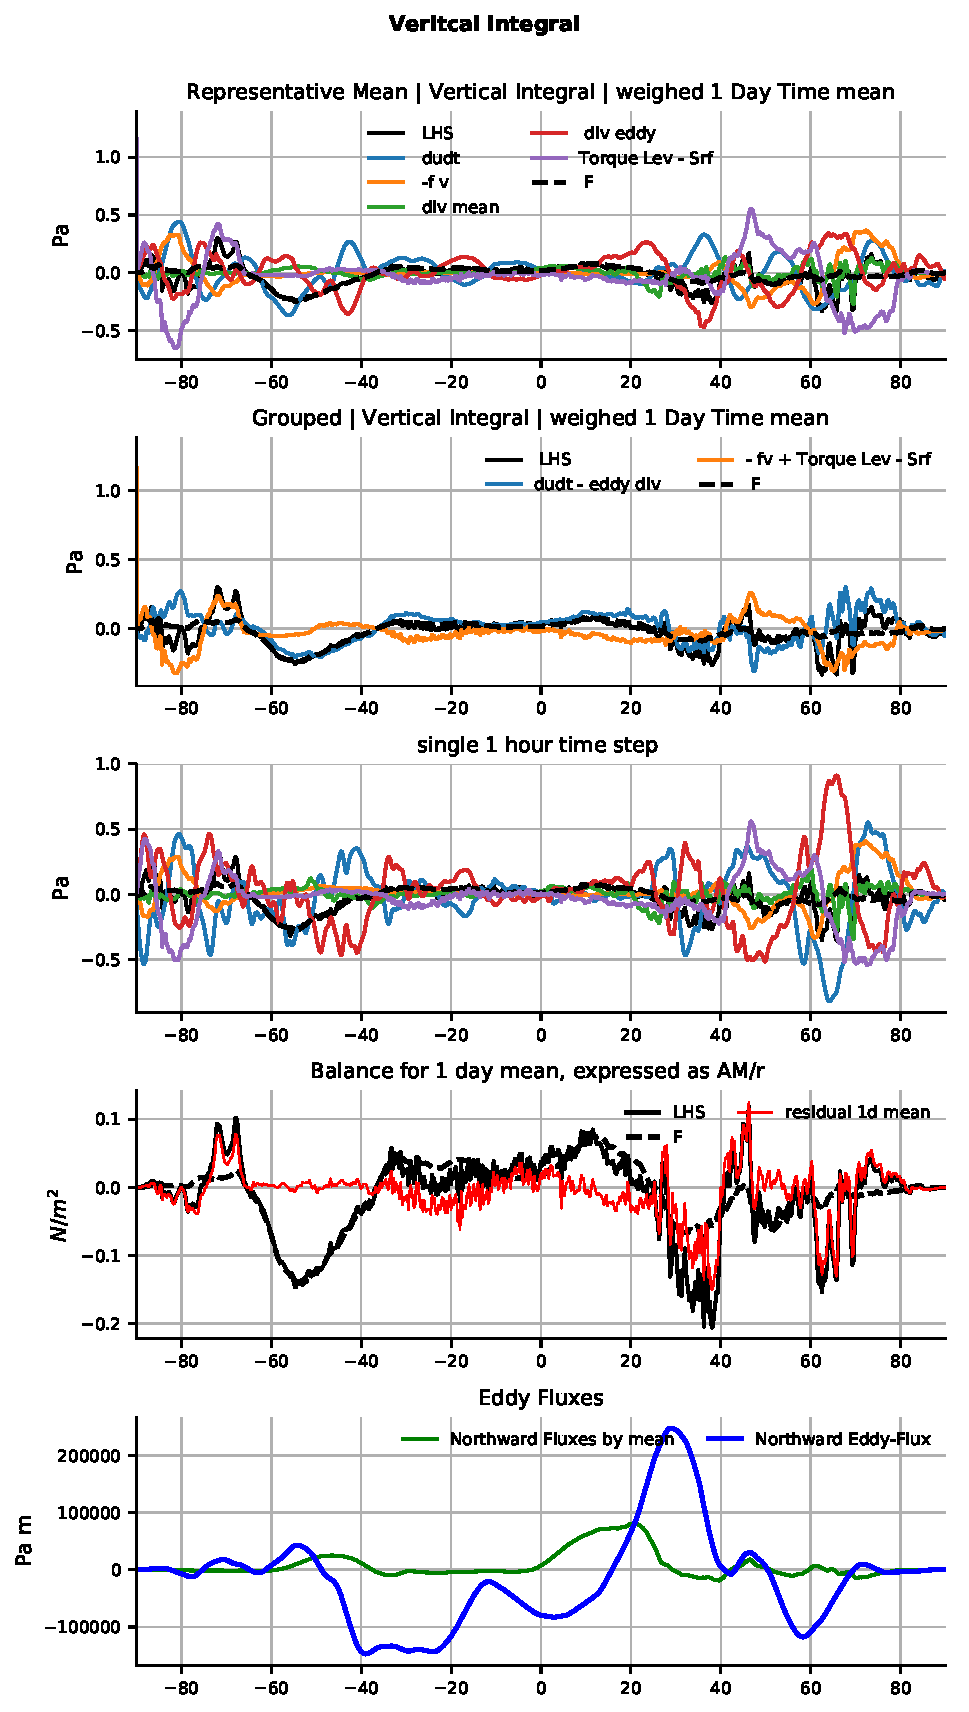
\includegraphics[scale=.7]{exmpl_repres_dmean_ps_iews_2000-01-18.pdf}}
\caption{Example the budget calculation of one day (2000-01-18) .}
\label{fig:AM_example1}
\end{figure}

\begin{figure}[h!]
\centerline{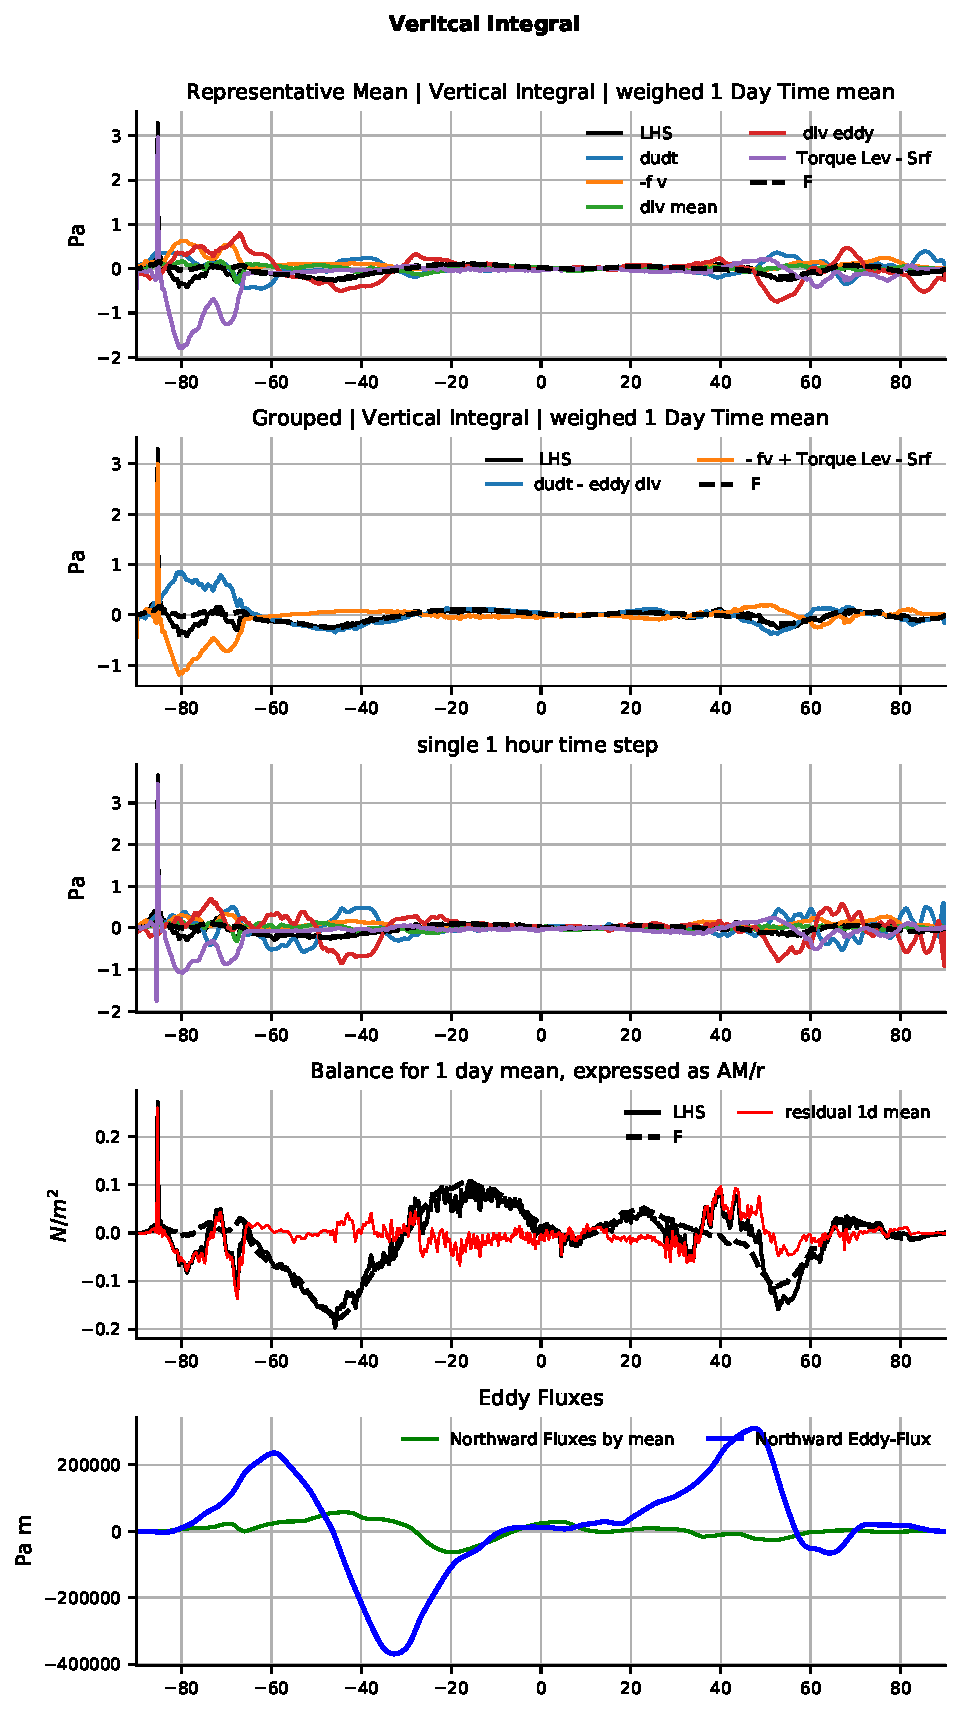
\includegraphics[scale=.7]{exmpl_repres_dmean_ps_iews_2005-09-28.pdf}}
\caption{Example the budget calculation of one day (2005-09-28).}
\label{fig:AM_example2}
\end{figure}


\begin{figure}[h!]
\centerline{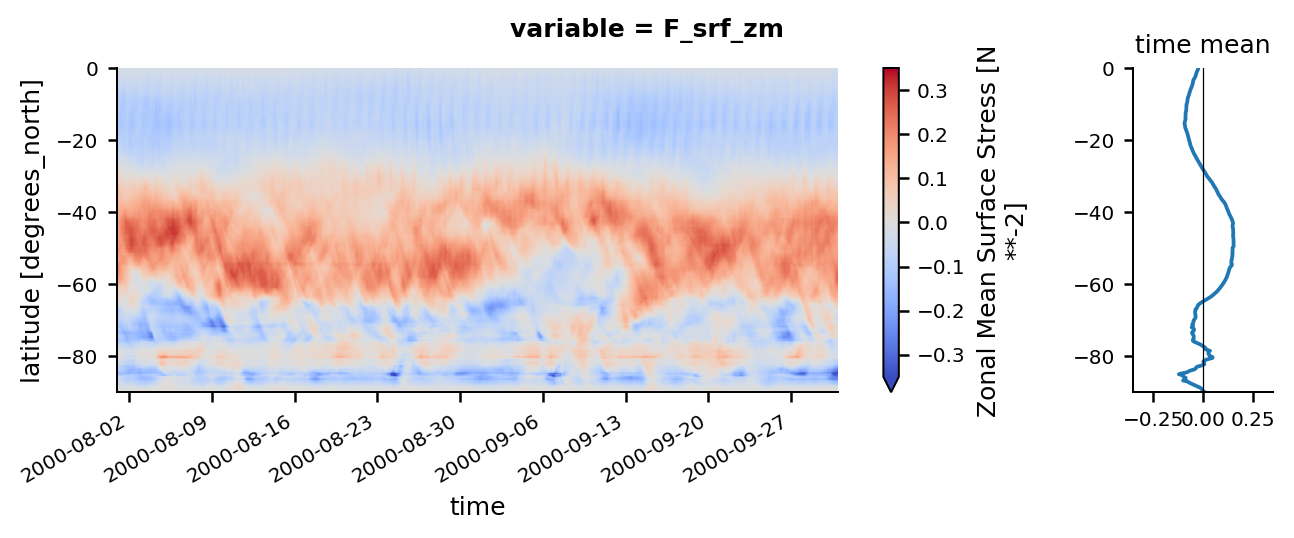
\includegraphics[scale=.8]{F_srf_zm.png}}
\caption{Zonal mean surface stress over the Southern Hemisphere.}
\label{fig:AM_example3}
\end{figure}





%\subsection{Bibliography}
\bibliographystyle{agufull}%{agu}%{elsarticle-harv}%{agu}
\footnotesize
\bibliography{books,thesis_proposal,Angular_momentum_budget}

%\newpage

%\section{Python code code}
%\lstinputlisting[language=python, basicstyle=\tiny]{./mhell_HW1_nr2.py}

%\lstinputlisting[language=matlab]{./testode.m}


%%%%%%%%%%%%%%%%%%%%%%%%
%%%%%%%%%%%  FIGURE %%%%%%%% 
%%%%%%%%%%%%%%%%%%%%%%%%
%\begin{figure}
%\epsfig{file=averagingComparison,width=0.9\textwidth}
%\caption{Comparison of the numerical solution of \eqref{cubedamp1} with the approximate solution in \eqref{approxSol}. Even though %\beta =1$ there is good agreement between the approximate solution \eqref{approxSol} and the \texttt{matlab} numerical solution.}
%\label{Fig1}
%\end{figure}
%%%%%%%%%%%%%%%%%%%%%%
%%%%%%%%%%%  FIGURE %%%%%%



%\clearpage

%\begin{verbatim}


%\end{verbatim}





\end{document}   
